\section{Conclusion}

\subsection{Explanatory Visualization}
Since I have already visualized a big part of the machine learning pipeline implemented during this project in the previous sections (like the clustering results or the structure of the principal components), I have decided to provide a visualization of the purpose of the predictor created during the project and its function within the overall framework that is the motivation for the project. This visualization is given in Fig.~\ref{fig_expl_viz}. In the completed framework, the computer science tutor who is designing the exercise for his/her course provides information about the students in the class, the problem, i.e., the subject of the exercise, and the exercise structure. I think it is important to highlight that the results of this project are not limited to the trained student clusterer. In addition to the clusterer, the project results also propose a way for the tutor to describe the students by just two intuitive features (the two PCs, one describing the general correctness and the other one describing the time needed to process the problems).  

 \begin{figure}
 	\centering
 	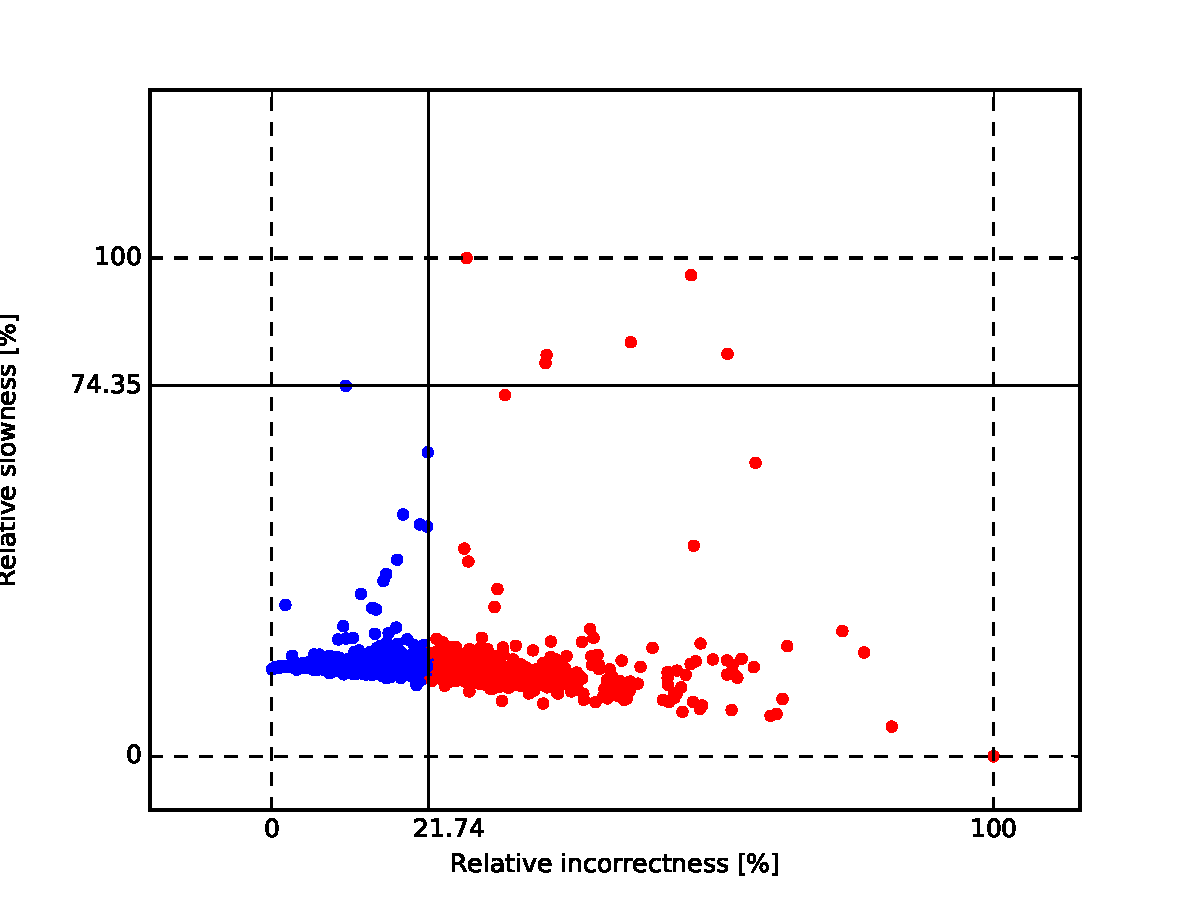
\includegraphics[width=\textwidth]{./img/explViz.pdf}
 	\caption{Illustration of the overall framework for the exercise design. The parts with a blue filling were implemented within this project, while the parts with gray filling and a dotted border are subjects of future work.\label{fig_expl_viz}}
 \end{figure}

\subsection{Recap of the Learning Experience}
Beside the practice that I got using the sklearn and the pandas frameworks, there were several practical insights I got through this project, where I had to apply machine learning techniques to the solution of a real problem, working with real data:

\begin{itemize}
	\item \textbf{Evaluation:} In the other projects of the nanodegree, the evaluation metric was mostly clearly defined and unambiguous, in that a model with an optimal result in this metric was actually the best one to solve the problem. However, in the capstone project, there was no given evaluation metric and the metric that I found myself, in the best case, had a mere correlation with the quality of the model. This makes the design of the predictor more challenging, as the effect on the model's usefulness for the problem cannot be directly read from the evaluation function and each decision, consequently has to be carefully considered by, e.g., looking at the resulting visualizations. However, I do think that this is a challenge that occurs frequently, especially during the application of unsupervised learning techniques. Working on this project definitely gave me valuable experience for these situations.
	\item \textbf{Importance of Visualization:} When choosing the number of principal components, I ended up using just two, although they explained only 70\% of the variance. However, using two PCs enabled a very comprehensive evaluation, where I could immediately see the effect of certain design decisions. Before working on this project, I would not have expected a case where a decision with worse performance values (like the explained variance) could be preferable. During the project, I definitely learned the importance of visualization. 
	\item \textbf{Importance of Practical Aspects:} Similarly to the point with the visualization, there were several other points in the project where I accepted information loss or a decision with a worse performance metric because it was more practical for other components of the pipeline or for the actual usage in the overall framework. For example, it may have been interesting to examine how the clustering algorithms would perform without a prior PCA step. However, even in the case where the predictors trained with more features would be more accurate, they would be impractical for the tutors, as the tutors would have to provide a very big number of specific characteristics about a student to obtain a classification. With this project, I learned that, for certain decisions, practicality with respect to the underlying problem may outweigh a better performance score when designing a machine learning pipeline for a real, practical problem.
\end{itemize}

\subsection{Possible Improvements}
Although I think that the pipeline created during this project could already be used within a framework for exercise design, there are several opportunities for further improvement:

\begin{itemize}
	\item \textbf{Using the entire Framework as Benchmark:} Overall, the student classification is intended to be a part of the framework for the exercise design. Consequently, each design decision should be evaluated by measuring its effect on the the classification of the teaching effect of the exercises. After the development of the other parts of the framework, the design decisions made for the student classifier should be reviewed with respect to their effect on the exercise classification.
	\item \textbf{Using the Problem View Feature:} I did not come up with a good way to average over the problem view feature that indicated how often a student has seen a problem. I do, however, definitely think that this feature is important for the student classification, as solving a problem correctly becomes easier when the problem was encountered before. Finding a way to average over this feature and considering the feature during the clustering may provide better results during the student clustering. 
	\item \textbf{Using the KC features/the problem classification:} I did not use the KC features as I suspected them to be specific to the area of math problems. However, using them may provide a stronger distinction between the different problems and their difficulty. An alternative way to incorporate the difficulty of the problem would be to use the results of the problem clustering as an additional feature for the student clustering.
\end{itemize}


\subsection{Project Summary}
Within this project, I have created a predictor that estimates whether a student is rather very or rather less able. During the preprocessing, I mapped the features from the original set onto two new hidden features, describing how correctly students solve the tasks as well as how much time they need to come up with a solution. Both these new features can be easily used by a tutor to describe the students in his/her class. The software can be used to create labels for the students in the data set and to use these labels to train a framework for the prediction of the effectiveness of an exercise.  